\documentclass{article}
\usepackage[utf8]{inputenc}
\usepackage{amssymb}
\usepackage{amsmath}
\usepackage{amsfonts}
\usepackage{mathtools}
\usepackage{hyperref}
\usepackage{fancyhdr, lipsum}
\usepackage{ulem}
\usepackage{fontspec}
\usepackage{xeCJK}
\setCJKmainfont[Path = /usr/share/fonts/TTF/]{edukai-5.0.ttf}
\usepackage{physics}
% \setCJKmainfont{AR PL KaitiM Big5}
% \setmainfont{Times New Roman}
\usepackage{multicol}
\usepackage{zhnumber}
% \usepackage[a4paper, total={6in, 8in}]{geometry}
\usepackage[
	a4paper,
	top=2cm, 
	bottom=2cm,
	left=2cm,
	right=2cm,
	includehead, includefoot,
	heightrounded
]{geometry}
% \usepackage{geometry}
\usepackage{graphicx}
\usepackage{xltxtra}
\usepackage{biblatex} % 引用
\usepackage{caption} % 調整caption位置: \captionsetup{width = .x \linewidth}
\usepackage{subcaption}
% Multiple figures in same horizontal placement
% \begin{figure}[H]
%      \centering
%      \begin{subfigure}[H]{0.4\textwidth}
%          \centering
%          \includegraphics[width=\textwidth]{}
%          \caption{subCaption}
%          \label{fig:my_label}
%      \end{subfigure}
%      \hfill
%      \begin{subfigure}[H]{0.4\textwidth}
%          \centering
%          \includegraphics[width=\textwidth]{}
%          \caption{subCaption}
%          \label{fig:my_label}
%      \end{subfigure}
%         \caption{Caption}
%         \label{fig:my_label}
% \end{figure}
\usepackage{wrapfig}
% Figure beside text
% \begin{wrapfigure}{l}{0.25\textwidth}
%     \includegraphics[width=0.9\linewidth]{overleaf-logo} 
%     \caption{Caption1}
%     \label{fig:wrapfig}
% \end{wrapfigure}
\usepackage{float}
%% 
\usepackage{calligra}
\usepackage{hyperref}
\usepackage{url}
\usepackage{gensymb}
% Citing a website:
% @misc{name,
%   title = {title},
%   howpublished = {\url{website}},
%   note = {}
% }
\usepackage{framed}
% \begin{framed}
%     Text in a box
% \end{framed}
%%

\usepackage{array}
\newcolumntype{F}{>{$}c<{$}} % math-mode version of "c" column type
\newcolumntype{M}{>{$}l<{$}} % math-mode version of "l" column type
\newcolumntype{E}{>{$}r<{$}} % math-mode version of "r" column type
\newcommand{\PreserveBackslash}[1]{\let\temp=\\#1\let\\=\temp}
\newcolumntype{C}[1]{>{\PreserveBackslash\centering}p{#1}} % Centered, length-customizable environment
\newcolumntype{R}[1]{>{\PreserveBackslash\raggedleft}p{#1}} % Left-aligned, length-customizable environment
\newcolumntype{L}[1]{>{\PreserveBackslash\raggedright}p{#1}} % Right-aligned, length-customizable environment

% \begin{center}
% \begin{tabular}{|C{3em}|c|l|}
%     \hline
%     a & b \\
%     \hline
%     c & d \\
%     \hline
% \end{tabular}
% \end{center}    



\usepackage{bm}
% \boldmath{**greek letters**}
\usepackage{tikz}
\usepackage{titlesec}
% standard classes:
% http://tug.ctan.org/macros/latex/contrib/titlesec/titlesec.pdf#subsection.8.2
 % \titleformat{<command>}[<shape>]{<format>}{<label>}{<sep>}{<before-code>}[<after-code>]
% Set title format
% \titleformat{\subsection}{\large\bfseries}{ \arabic{section}.(\alph{subsection})}{1em}{}
\usepackage{amsthm}
\usetikzlibrary{shapes.geometric, arrows}
% https://www.overleaf.com/learn/latex/LaTeX_Graphics_using_TikZ%3A_A_Tutorial_for_Beginners_(Part_3)%E2%80%94Creating_Flowcharts

% \tikzstyle{typename} = [rectangle, rounded corners, minimum width=3cm, minimum height=1cm,text centered, draw=black, fill=red!30]
% \tikzstyle{io} = [trapezium, trapezium left angle=70, trapezium right angle=110, minimum width=3cm, minimum height=1cm, text centered, draw=black, fill=blue!30]
% \tikzstyle{decision} = [diamond, minimum width=3cm, minimum height=1cm, text centered, draw=black, fill=green!30]
% \tikzstyle{arrow} = [thick,->,>=stealth]

% \begin{tikzpicture}[node distance = 2cm]

% \node (name) [type, position] {text};
% \node (in1) [io, below of=start, yshift = -0.5cm] {Input};

% draw (node1) -- (node2)
% \draw (node1) -- \node[adjustpos]{text} (node2);

% \end{tikzpicture}

%%

\DeclareMathAlphabet{\mathcalligra}{T1}{calligra}{m}{n}
\DeclareFontShape{T1}{calligra}{m}{n}{<->s*[2.2]callig15}{}

% Defining a command
% \newcommand{**name**}[**number of parameters**]{**\command{#the parameter number}*}
% Ex: \newcommand{\kv}[1]{\ket{\vec{#1}}}
% Ex: \newcommand{\bl}{\boldsymbol{\lambda}}
\newcommand{\scripty}[1]{\ensuremath{\mathcalligra{#1}}}
% \renewcommand{\figurename}{圖}
\newcommand{\sfa}{\text{  } \forall}
\newcommand{\floor}[1]{\lfloor #1 \rfloor}
\newcommand{\ceil}[1]{\lceil #1 \rceil}


%%
%%
% A very large matrix
% \left(
% \begin{array}{ccccc}
% V(0) & 0 & 0 & \hdots & 0\\
% 0 & V(a) & 0 & \hdots & 0\\
% 0 & 0 & V(2a) & \hdots & 0\\
% \vdots & \vdots & \vdots & \ddots & \vdots\\
% 0 & 0 & 0 & \hdots & V(na)
% \end{array}
% \right)
%%

% amsthm font style 
% https://www.overleaf.com/learn/latex/Theorems_and_proofs#Reference_guide

% 
%\theoremstyle{definition}
%\newtheorem{thy}{Theory}[section]
%\newtheorem{thm}{Theorem}[section]
%\newtheorem{ex}{Example}[section]
%\newtheorem{prob}{Problem}[section]
%\newtheorem{lem}{Lemma}[section]
%\newtheorem{dfn}{Definition}[section]
%\newtheorem{rem}{Remark}[section]
%\newtheorem{cor}{Corollary}[section]
%\newtheorem{prop}{Proposition}[section]
%\newtheorem*{clm}{Claim}
%%\theoremstyle{remark}
%\newtheorem*{sol}{Solution}



\theoremstyle{definition}
\newtheorem{thy}{Theory}
\newtheorem{thm}{Theorem}
\newtheorem{ex}{Example}
\newtheorem{prob}{Problem}
\newtheorem{lem}{Lemma}
\newtheorem{dfn}{Definition}
\newtheorem{rem}{Remark}
\newtheorem{cor}{Corollary}
\newtheorem{prop}{Proposition}
\newtheorem*{clm}{Claim}
%\theoremstyle{remark}
\newtheorem*{sol}{Solution}

% Proofs with first line indent
\newenvironment{proofs}[1][\proofname]{%
  \begin{proof}[#1]$ $\par\nobreak\ignorespaces
}{%
  \end{proof}
}
\newenvironment{sols}[1][]{%
  \begin{sol}[#1]$ $\par\nobreak\ignorespaces
}{%
  \end{sol}
}
%%%%
%Lists
%\begin{itemize}
%  \item ... 
%  \item ... 
%\end{itemize}

%Indexed Lists
%\begin{enumerate}
%  \item ...
%  \item ...

%Customize Index
%\begin{enumerate}
%  \item ... 
%  \item[$\blackbox$]
%\end{enumerate}
%%%%
% \usepackage{mathabx}
\usepackage{xfrac}
%\usepackage{faktor}
%% The command \faktor could not run properly in the pc because of the non-existence of the 
%% command \diagup which sould be properly included in the amsmath package. For some reason 
%% that command just didn't work for this pc 
\newcommand*\quot[2]{{^{\textstyle #1}\big/_{\textstyle #2}}}


\makeatletter
\newcommand{\opnorm}{\@ifstar\@opnorms\@opnorm}
\newcommand{\@opnorms}[1]{%
	\left|\mkern-1.5mu\left|\mkern-1.5mu\left|
	#1
	\right|\mkern-1.5mu\right|\mkern-1.5mu\right|
}
\newcommand{\@opnorm}[2][]{%
	\mathopen{#1|\mkern-1.5mu#1|\mkern-1.5mu#1|}
	#2
	\mathclose{#1|\mkern-1.5mu#1|\mkern-1.5mu#1|}
}
\makeatother
% \opnorm{a}        % normal size
% \opnorm[\big]{a}  % slightly larger
% \opnorm[\Bigg]{a} % largest
% \opnorm*{a}       % \left and \right



\linespread{1.5}
\pagestyle{fancy}
\title{普通天文學2024作業二}
\author{B11202041 物理二 $ $ 劉晁泓}
% \date{\today}
\date{March 23, 2024}
\begin{document}
\maketitle
\thispagestyle{fancy}
\renewcommand{\footrulewidth}{0.4pt}
\cfoot{\thepage}
\renewcommand{\headrulewidth}{0.4pt}
\fancyhead[L]{普通天文學2024作業二}

\setlength{\parindent}{0pt}
Note:本作業請使用太陽質量($1.989 \cdot 10^{30}$ kg)為所有質量的單位\\
$M_{\text{sun}} \rightarrow$ 太陽質量\\
Mpc $\rightarrow 10^6$ pc\\
$\text{AU} \rightarrow 1.5 \cdot 10^8$ km

\setlength{\parindent}{20pt}
\begin{enumerate}
	\item[1.] [10分]課上我們提到暗物質佔目前宇宙整體能量約25\%,
		但是有趣的是,
		在我們日常生活或是太陽系中抑或是地球的運行軌道,
		好像沒有感受到暗物質所提供的重力,
		我們可以透過以下計算來了解暗物質在太陽系尺度下所產生的重力效應。\\
		\par 下圖為銀河系中預期的暗物質密度隨著銀河系中心距離的變化,
		太陽系約位於銀河系8 kpc的位置,
		相對應的按物質質量密度約$6 \cdot 10^6$ ($M_{\text{sun}}/\text{kpc}^3$)。
		根據此資訊,
		估算在地球距離太陽半徑(1AU)的球體積裡,
		暗物質所佔的質量為何(以太陽質量為單位)?

		\begin{figure}[h]
			\centering
			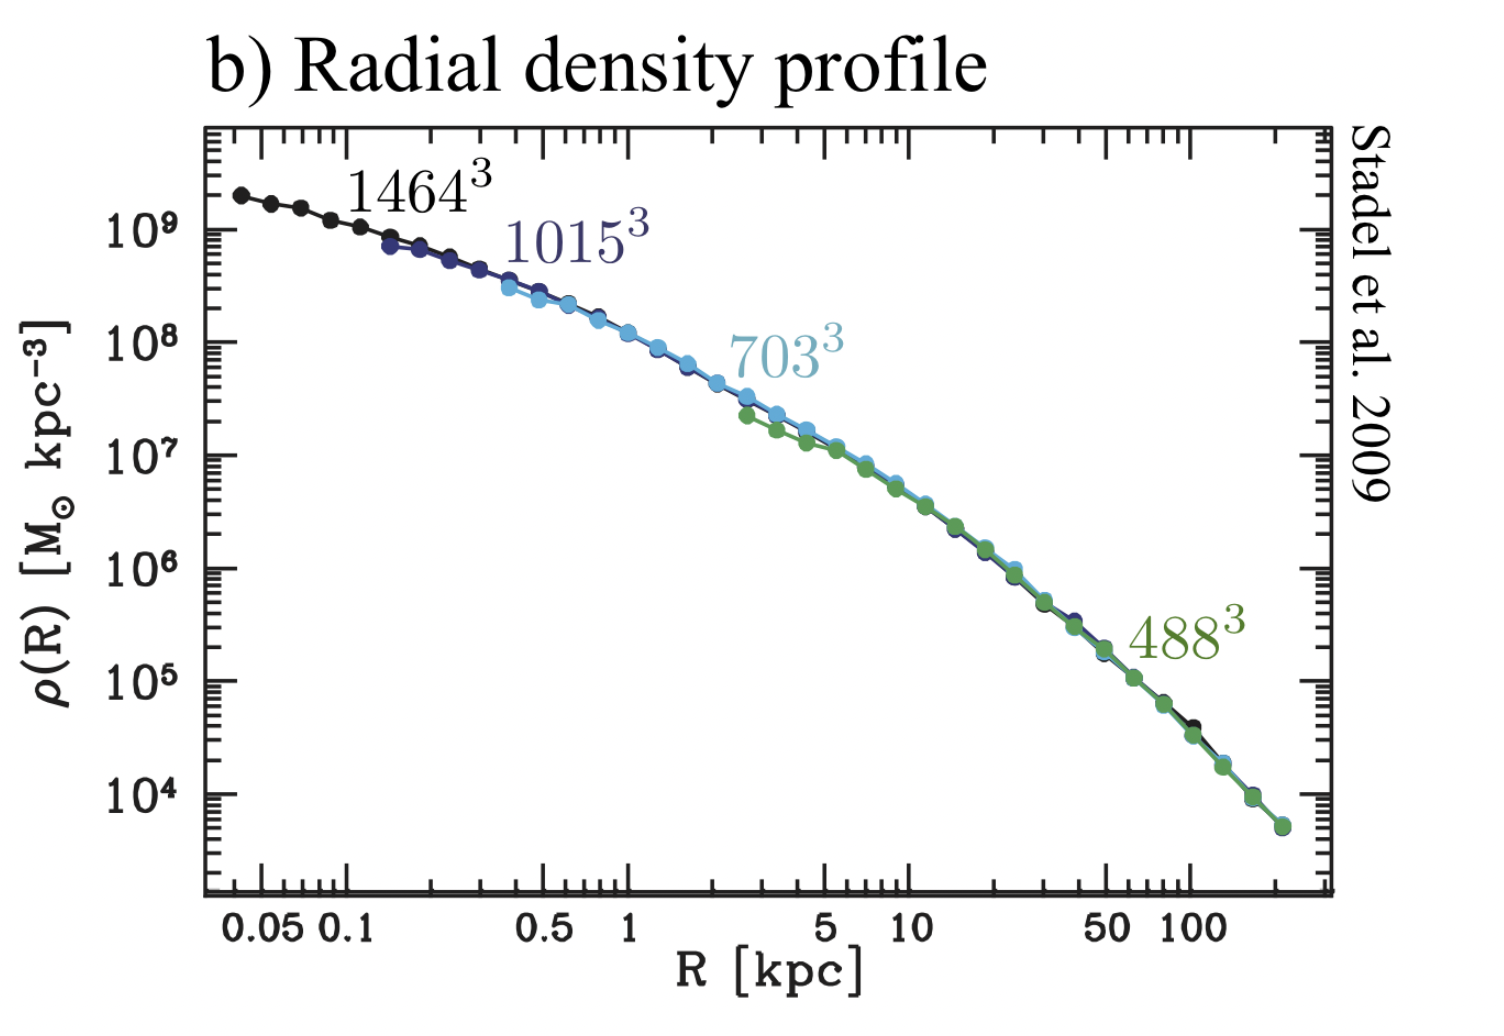
\includegraphics[scale = 0.2]{hw2-1.png}
			\caption{\url{https://arxiv.org/pdf/1404.1938.pdf}}
			\label{fig1}
		\end{figure}

	\item[1.] 解:\\
		記總質量為$M$,密度為$\rho$,體積為$V$,則
		\[
			M = V \rho = \frac{4 \pi}{3} (1 \text{AU})^3 \cdot 6 \cdot 10^6 (\frac{M_{\text{sun}}}{\text{kpc}^3}) = 8 \cdot 10^6 \pi \left( \frac{\text{AU}}{\text{kpc}} \right)^3 M_{\text{sun}} = 2.864 \cdot 10^{-18} M_{\text{sun}}
		\]
		這裡使用了$1 \text{kpc} = 10^3 \cdot 206265 \text{AU}$。

	\item[2.] [10分][圖來自COBE衛星]上課講到COBE衛星觀測CMB,
		將平均值減掉後,
		得到上圖的溫度差,
		根據COBE的結果溫度差為3.3 mK(深紅色是比平均多$\sim 3.3$ mK,
		深藍色是比平均少$\sim 3.3$ mK)。
		根據這個溫度,
		推算出太陽系相對CMB的速度為何?
		[提示如果根據Wien's law,
		溫度變化同等於波長變化,
		波長變化跟速度有關(都普勒效應)]

		\begin{figure}[h]
			\centering
			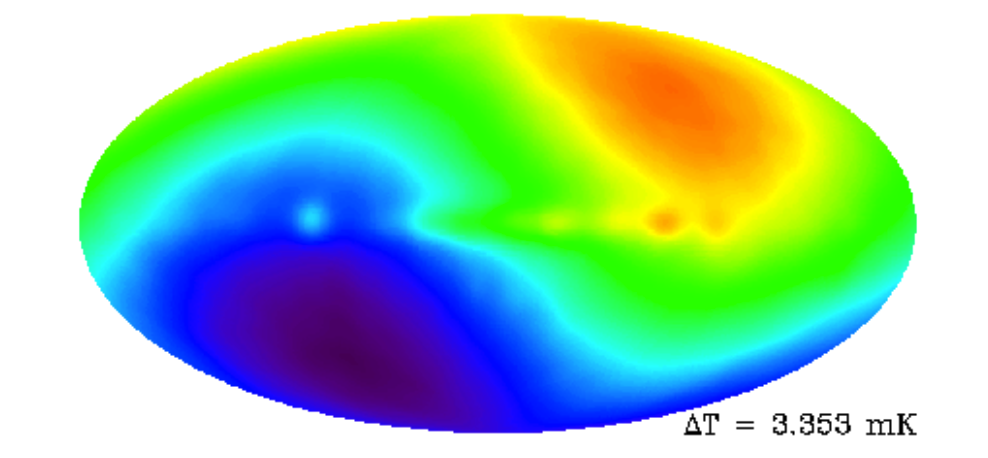
\includegraphics[scale = 0.3]{hw2-2.png}
			\caption{}
			\label{fig2}
		\end{figure}

	\item[2.] 解:\\
		這裡我們使用Wien's Law:
		\[
			\lambda T = 0.29 (\text{cm} \cdot \text{K})
		\]
		根據宇宙背景輻射的溫度$2.73$K,
		我們可以推算出應該要測量到的波長$\lambda_{\text{CMB}}$
		\[
			\lambda_{\text{CMB}} = \frac{0.29}{2.73} (\text{cm}) = 0.106227 \text{ cm}
		\]
		但今天我們在太陽系測到了溫度$T$與CMB的溫度$T_{\text{CMB}}$差了3.3mK,
		因此我們可以推算量到的CMB的波長峰值$\lambda$
		\[
			\lambda = \frac{0.29}{2.7333} (\text{cm}) = 0.106989 \text{ cm}
		\]
		因此根據都普勒效應,CMB的速率$v$與光速$c$的比值應有
		\[
			\frac{v}{c} \sim \frac{\lambda}{\lambda_{\text{CMB}}} - 1 = 7.17 \cdot 10^{-3}
		\]
		\[
			\Rightarrow v = 7.17 \cdot 10^{-3} c
		\]

	\item[3.] [30分]Zwicky當初觀測星系團中的星系的相對速度,
		計算所需要的質量,
		發現暗物質。
		請使用此觀測資料(\href{https://www.dropbox.com/s/6z5jypo7tj2ulen/Virgo_galaxy_catalog.csv?dl=0}{Virgo\_galaxy\_catalog.csv}),
		按照以下步驟做一樣的運算。

		\begin{figure}[h]
			\centering
			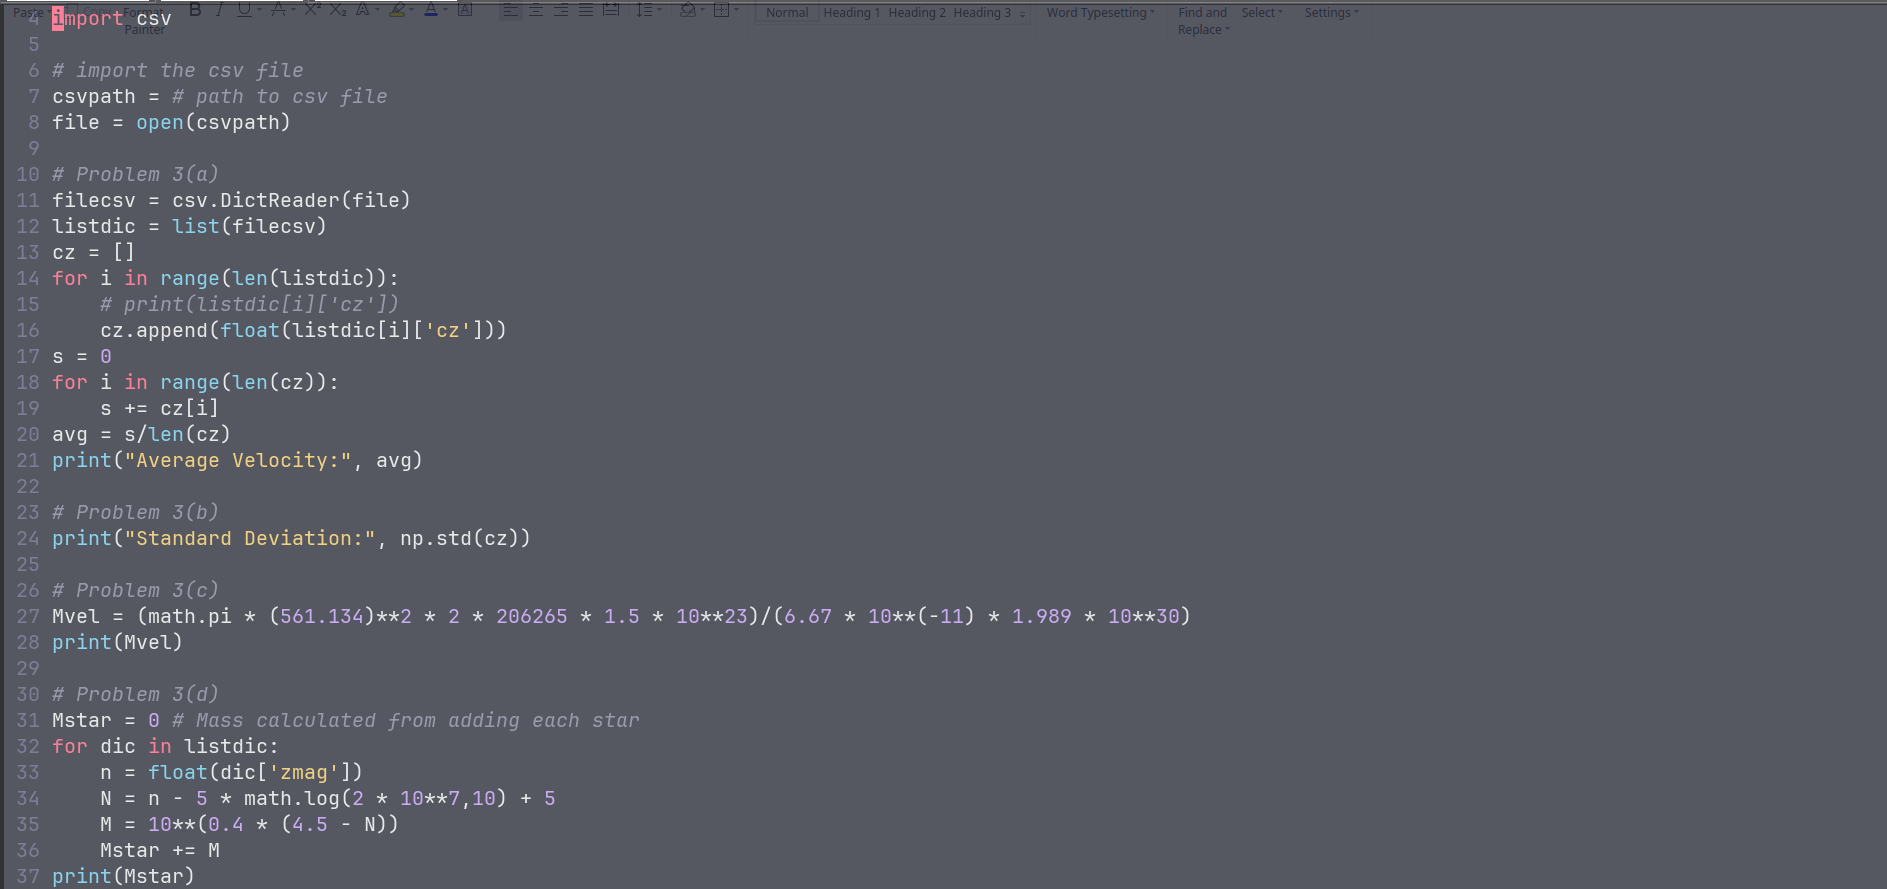
\includegraphics[scale = 0.25]{hw2-3.png}
			\caption{第三題程式碼截圖}
			\label{fig3}
		\end{figure}


		\begin{enumerate}
			\item[(a)] 該數據中有一個"cz"的欄位,
				代表的是那些星系相對太陽系的速度,
				單位km/s。
				請問在該星系團中所有的星系相對太陽系的平均速度為何?

			\item[(a)] 解:\\
				利用python讀取csv資料,
				並計算cz行的速度的平均值$v_{\text{avg}}$。
				如Fig \ref{fig3}中3(a)部份的程式碼。
				\[
					v_{\text{avg}} = 1036.195 \text{ km/s}
				\]

			\item[(b)] cz有一個分佈,
				請問根據數據所計算出來的cz標準差為何?

			\item[(b)] 解:\\
				利用numpy中np.std()函數計算標準差。
				如Fig \ref{fig3}中3(b)部份的程式碼。
				\[
					\sigma = 561.134 \text{ km/s}
				\]

			\item[(c)] 此標準差值,
				在天文稱為velocity dispersion($\sigma$),
				跟系統內的質量有以下關係($M$為質量)
				\[
					M \simeq \frac{\pi \sigma^2 R}{G}
				\]
				其中$R$是星系團半徑約2 Mpc,
				$G$為重力常數。
				計算該星系團的質量。

			\item[(c)] 解:\\
				如Fig \ref{fig3}中3(c)部份的程式碼。
				\[
					M = \frac{\pi \cdot (561.134 \cdot 10^3)^2 \cdot 2 \cdot 10^6 \cdot 206265 \cdot (1.5 \cdot 10^{11})}{6.67 \cdot 10^{-11} \cdot 1.989 \cdot 10^{30}} (M_{\text{sun}}) = 4.614 \cdot 10^{14} M_{\text{sun}}
				\]

			\item[(d)] 該數據中有一個"zmag"的欄位,
				代表那些星系用SDSS z band filter的觀測星等,
				這個星系團離我們的距離為20 Mpc,
				先計算這些星系的絕對星等。
				接著計算這些星系相對於太陽有多亮
				(太陽在z band的絕對星等為4.5)。
				假設星系的光度相對於太陽的光度,
				約等於星系的質量相對於太陽的質量
				(天文稱這個為mass to light ratio),
				計算在這個目錄內所有星系的質量加總。
				這個數星星算出來的質量,
				跟用速度算出來的質量差多少?
				[可以使用任何能幫助你做計算的工具(Excel, google sheet, python, matlab)等等]
				請附上你所使用的程式碼截圖。
				[資料來源:\href{https://ui.adsabs.harvard.edu/abs/2015yCat..22150022K/abstract}{資料1}]

			\item[(d)] 解:\\
				(這題中使用$n, N$代表星等以免與質量搞混)
				這些星系的絕對星等$N$與觀測星等$n$的關係為
				\[
					N = n - 5 \log_{10} \frac{d}{\text{pc}} + 5 = n - 5 \log_{10} (2 \cdot 10^7) + 5
				\]
				設太陽的光度為$L_{\text{sun}}$,絕對星等為$N_{\text{sun}}$,則我們有
				\[
					N - N_{\text{sun}} = -2.5 \log_{10} \frac{L}{L_{\text{sun}}}
				\]
				\[
					\Rightarrow \frac{M}{M_{\text{sun}}} = \frac{L}{L_{\text{sun}}} = 10^{0.4 (N_{\text{sun}} - N)}
				\]
				最後我們將所有的$M/M_{\text{sun}}$求和,得到總質量$M_{\text{star}} = 3.304 \cdot 10^{12}$ ($M_{\text{sun}}$),
				發現與用速度算的差了約140倍。
				如Fig \ref{fig3}中3(d)部份的程式碼。
		\end{enumerate}

	\item[4.] [20分]根據宇宙大霹靂理論,
		宇宙年齡約38萬年的時候,
		溫度下降到3000 K,
		光子無法將電子從中性氫中游離開來,
		
		\begin{enumerate}
			\item[(a)] 將電子完全從氫氣游離的能量為13.6 eV,
				試問相對應的光子波長為何?

			\item[(a)] 解:
				\[
					\lambda = \frac{h c}{E} = \frac{6.626 \cdot 10^{-34} \cdot 299792458}{13.6 \cdot 1.602 \cdot 10^{-19}} = 9.117 \cdot 10^{-8} \text{ m} = 9.117 \cdot 10^{-6} \text{ cm} 
				\]

			\item[(b)] 根據黑體輻射Wien's law,
				該光子波長相對應的溫度又是如何?

			\item[(b)] 解:\\
				\[
					T = \frac{0.29}{9.117 \cdot 10^{-6}} = 31808 \text{ K} 
				\]
			\item[(c)] 請解釋為何不是當宇宙下降到13.6 eV相對應的溫度時,
				光子就無法將電子從中性氫中游離開來,
				為何需要下降到3000 K?

			\item[(c)] 解:\\
				當宇宙中存在一團密度很高的電子與質子時,
				電子受到的力不只有質子的吸引力,
				還要考慮與其他電子的排斥力,
				這會讓質子的束縛能下降許多,
				讓電子非常容易游離,
				需要更低的溫度把電子放回能階上。

		\end{enumerate}

	\item[5.] [15分] 請看這個\href{https://www.youtube.com/watch?v=JmDszPExepc&ab_channel=issiber}{演講}by Adam Riess [\textbf{1 hour!}],
		根據演講內容回答以下問題。

		\begin{enumerate}
			\item[(a)] 聽完這個演講,
				有哪些東西是你上完這前三週的課之後,
				可以聽得懂的?[100字以內]

			\item[(a)] 解:\\
				這篇演講基本上都是在講測量哈伯常數時,
				與在校正距離階梯(distance ladder)時的具體作為。
				前面在講述他的動機,
				現行的$\Lambda$CDM模型與觀測的互相校正,
				距離階梯中的視差法、造父變星等都是聽得懂的。

			\item[(b)] 聽完這個演講,
				有哪些東西是你沒有聽懂的?[100字以內]

			\item[(b)] 解:\\
				後面在講述Ia supernovae的一些細節校正,
				與這些校正的研究結果時,
				因為不太清楚這個方法具體是怎麼進行的,
				所以很多專有名詞沒有很懂,
				只能看拼成一整條線的宇宙距離階梯圖大致上猜測他在幹嘛。

			\item[(c)] 演講中提及用標準燭光所計算的哈伯常數,
				可能會造成系統性誤差的原因有哪些?
				那講者是如何用資料來測試可能的系統性誤差?

			\item[(c)] 在測量造父變星的光度時,
				他們盡可能觀測不同星系的造父變星,
				選擇周遭組成物質相近的系統,
				並且壓短觀測時間以降低灰塵變化造成的影響等。

		\end{enumerate}

	\item[6.] 上課提到透過CMB偵測暴漲的訊號。
		在2014年,
		一組天文團隊叫BICEP2公佈他們偵測到暴漲的訊號,
		請讀以下\href{https://physicsworld.com/a/bicep2-finds-first-direct-evidence-of-cosmic-inflation/#:~:text=The\%20first\%20evidence\%20for\%20the,telescope\%20at\%20the\%20South\%20Pole.}{文章}關於他們的研究成果,
		接著請讀\href{https://phys.org/news/2015-02-cosmic-inflation-bicep2-results.html}{此文章},
		並回答以下問題。
		\begin{enumerate}
			
			\item[(a)] 要偵測暴漲的CMB訊號,
				文章中提到要透過一種polarization的訊號,
				請寫出他的名稱。

			\item[(a)] 解:\\
				此訊號為primordial B-mode polarization的訊號。

			\item[(b)] 請問當初BICEP2認為他們有偵測到暴漲的訊號,
				後來發現該訊號是其他東西所造成的,
				請問那個東西是什麼?

			\item[(b)] 解:\\
				根據這篇\href{https://www.nature.com/articles/nature.2015.16830}{Nature的文章}(2015年,針對BICEP2的評論),
				後來發現這個訊號是由宇宙中的灰塵所產生,
				研究團隊將352GHz的灰塵訊號與應在150GHz左右偵測到的primordial B-mode polarization訊號搞混了。

			\item[(c)] 讀完這些結果,
				請寫下你的心得[100字以內]。

			\item[(c)] 解:\\
				從這項研究的經驗看來,
				在發表重大實驗結果前應該要更仔細的確認是否真的每個環節都沒有出錯,
				有沒有跟以前的數據長得莫名其妙像等等,
				應該保持一個清醒的腦袋做研究。

		\end{enumerate}

	\item[7.] 請閱讀這篇\href{https://calteches.library.caltech.edu/638/2/Men.pdf}{文章}並寫下你的心得[100字以內]。
		[如果以上連結不能用,使用\href{https://www.dropbox.com/s/yggx7xfldi5fefj/prime_focus_cage_men.pdf}{連結2}]

	\item[7.] 解:\\
		這篇文章大致上幫助我瞭解天文學家的生活。
		其實大致上與我想像得差不多,
		基本上就是找個好天氣叫助理上去看星星,
		然後自己在下面做數據分析。
		這樣的生活樸實無華且會有點無聊,
		想必需要極大的熱誠才能堅持下去,
		原來這些堆出來的天文數據背後都是一些肝帝日夜觀察分析的結果,
		我們在用數據的時候應該抱持著飲水思源的心態感謝他們。


\end{enumerate}















\end{document}






